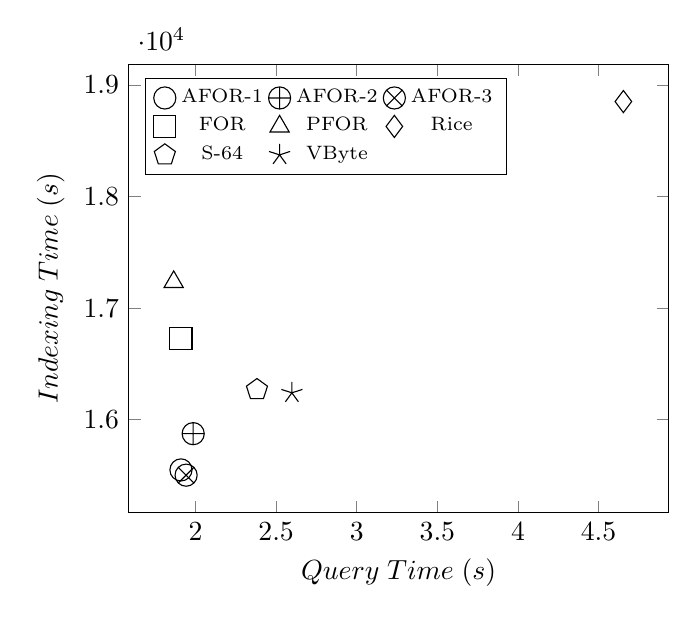
\begin{tikzpicture}
\begin{axis}[%
  scatter/classes={%
	a={mark=o},%
	b={mark=oplus},%
	c={mark=otimes},%
	d={mark=square},%
	e={mark=triangle},%
	f={mark=diamond},%
	g={mark=pentagon},%
	h={mark=star}
  },
  ylabel=$Indexing \; Time \; (s)$,
  xlabel=$Query \; Time \; (s)$,
  mark options={scale=2},
  legend columns=3,
  legend pos=north west,
  legend style={font=\scriptsize, anchor=north west, legend columns=3},
]

\addplot[only marks]
plot[scatter,scatter src=explicit symbolic]
coordinates {%
(1.9096, 15550) [a]
(1.9854, 15875) [b]
(1.9415, 15503) [c]
(1.9094, 16727) [d]
(1.8644, 17235) [e]
(4.654, 18852) [f]
(2.381, 16270) [g]
(2.5977, 16241) [h]
};%
\legend{AFOR-1, AFOR-2, AFOR-3, FOR, PFOR, Rice, S-64, VByte}
\end{axis}
\end{tikzpicture}